
\chapter{Terminology}
In all areas of research or vocation, there is terminology used that is specific to that field, and astronomy is no exception. Although this is not a treatise on the study of astronomy, it would serve you well to become acquainted with some of these terms.

\section{Disciplines of research}

You will hear terms such as \textit{astronomy, archaeoastronomy} and \textit{ethnoastronomy}. These terms can sometime become confusing so I will provide short definitions for them.

\subsection{Astronomy}
Astronomy is one of physical sciences and involves the systematic study of celestial objects and phenomena that originate outside the Earth's atmosphere. Astronomic data from various missions are recorded in catalogues for use within the scientific community. Within the field of study, there are various terms used, which are important to know in order to query and interpret the astronomical data you will encounter.

\subsubsection{Field of View}
The \textit{field of view} is the amount of sky that you are able to see and it is measured in degrees.  If we zoom in, we reduce the field of view. If we compare Figures~\ref{fig:fov60} and ~\ref{fig:fov13}, we see the same point of sky is in the centre, however, the image that looks closer has a lower field of view.

\begin{figure}[htbp]
	\centering
	\includegraphics[width=1\columnwidth]{fov60}
	\caption{stellarium displaying a 60$^{\circ}$ field of view.}
	\label{fig:fov60}
\end{figure}

\begin{figure}[htbp]
	\centering
	\includegraphics[width=1\columnwidth]{fov13}
	\caption{stellarium displaying a 13$^{\circ}$ field of view.}
	\label{fig:fov13}
\end{figure}

\subsubsection{Observation Location}
The observer location is the geographical position from where the celestial observation is being made. These are defined using latitude and longitude. For example, if you were viewing the sky from Newcastle Australia, your geographical location would be  32.9283$^{\circ}$ South, 151.7817$^{\circ}$ East. Rather than using the terms south and east, northern latitudes are positive and southern are negative. Likewise, east is positive and west is negative. Therefore, the geographical location for Newcastle would be -32.9283, +151.7817.  A western longitude can also be positive, however, the value is 360$^{\circ}$ - the western longitude. Eg, a longitude of -90$^{\circ}$ is also +270$^{\circ}$.

It is also possible to set the planet or celestial body you are viewing from. 
For example, Figure ~\ref{fig_JupiterFromIO} displays us looking at Jupiter with our observation location as its moon Io.

Another parameter is the altitude from where the observation is being made. 

\begin{figure}[ht]
	\centerline{\includegraphics[width=1\columnwidth]{JupiterFromIO.png}}
	\caption{\label{fig_JupiterFromIO}{A simulation of Jupiter being viewed with Io as the observation location.}}
\end{figure}

\subsubsection{Date time - ISO 8601}
The ISO 8601 date and time format is a standardised way of defining the exact date and time. The time zone is the time difference between local time and Coordinated Universal Time (UTC) and does not change with daylight saving. The exact time is specified by the year, month, day followed by time in hours (24 hour code), minutes, seconds and the time zone.  The time zone for UTC is "Z", meaning zero. The time zone is modified by changing the "Z" to hours and minutes, separated by a semicolon. For example,  midday on January 1, 2000 at UTC would be defined as "2000-01-01T12:00:00Z". Likewise, "2019-06-01T14:13:00+10:00" would be 1 June 2019 at 2:15pm in Sydney, which is 10 hours ahead of or earlier than UTC time. 

\subsubsection{Azimuth}
\textit{Azimuth} is the direction with respect to celestial north and is measured in degrees. If, for example, you were looking due south, the azimuth would be 180. East is 90 and west is -90 or +270. 

\subsubsection{Altitude}
The altitude is the angle you are looking up or down at and is measured in degrees. If you were looking directly up, the altitude would be 90 degrees. Similarly, horizontal is zero and down is -90.

\subsubsection{Celestial Coordinates}
In the same way we can define an exact location on the Earth using latitude and longitude, we define the location of celestial objects using the celestial coordinate system. Instead of longitude and latitude, we use the terms \textit{Right ascension} and \textit{Declination}. 

\subsubsection{Right Ascension}
Right Ascension, abbreviated to \textit{RA}, is the angular distance from the east of the First Point of Aries (hereafter FPOA), and is measured in hours, minutes and seconds, and is similar to the longitude on earth, except on the celestial sphere. This is basically how long it takes from the time FPOA is on the meridian (directly north or south) for the RA in question to be overhead. For example, if an object had a Right ascension of 3 Hours, it would mean that it would appear on the meridian three hours after FPOA was.  This is similar to the concept of time zones. In order to make calculations easier, we convert the RA to a digital angle by multiplying the number of hours by 15 (24 hours x 15 = 360$^{\circ}$) . Furthermore, we use decimals instead of minutes and seconds. eg, 90$^{\circ}$ 30' would be written 90.5$^{\circ}$. 

\subsubsection{Declination}
The declination is equivalent to the concept of latitude and is the angular distance a star is north or south of the celestial equator when it is on the meridian (in line with north / south).  

\subsection{Magnitude}
The magnitude is how bright a star is. Higher magnitudes mean a lower brightness.

\subsection{Atmosphere}
Atmosphere is the gas that surrounds us and makes the sky appear like daylight. If there was no atmosphere, the sky would appear dark, as it does on the moon, and you would be easily able to see stars during the day. stellarium gives us the option to hide the atmosphere, enabling us to see stars at any time. For example, Figure ~\ref{fig_with-atmosphere} shows the midday with normal atmosphere, whereas ~\ref{fig_no-atmosphere} shows the same sky without the atmosphere.

\begin{figure}[ht]
	\centerline{\includegraphics[width=1\columnwidth]{with-atmosphere.png}}
	\caption{\label{fig_with-atmosphere}{Midday showing the sky with atmosphere.}}
\end{figure}

\begin{figure}[ht]
	\centerline{\includegraphics[width=1\columnwidth]{no-atmosphere.png}}
	\caption{\label{fig_no-atmosphere}{Midday showing the sky with no atmosphere.}}
\end{figure}


\subsection{Ethnoastronomy}
Ethnoastronomy is a social science belonging to the discipline of ethnology and examines the way astronomy is practised in the context of a particular culture \cite{Salt2015}.

\subsection{Archaeoastronomy}
Archaeoastronomy is the study of how ancient civilisations understood the cosmos and in a sense very similar to ethnoastronomy.
``Broad public embrace of archaic astronomy probably began in the eighteenth
century with awareness of the summer solstice sunrise’s affiliation with Stonehenge" \cite[p.~263]{Krupp2015}.
Archaeoastronomers have used stellarium to generate an astronomical display from a location for a period sometime in the past \cite{zotti2014towards}.

\subsection{Astrology}
``Astrology, from the Greek, astro-logos, is the assumption that the stars and planets
contain meaning and significance for terrestrial affairs....Astrology appears to
be a universal feature of human culture and may be understood as a form of cultural
astronomy; an important contribution to the understanding of astronomy’s cultural
uses, applications, uses, and functions; and an indication of society’s attitudes to the
stars."\cite[p.~104]{Campion2015}. stellarium has a feature whereby you can display constellation art, as shown in ~\ref{fig_constellation-art}, which facilitates representing astrology in your works.

\begin{figure}[ht]
	\centerline{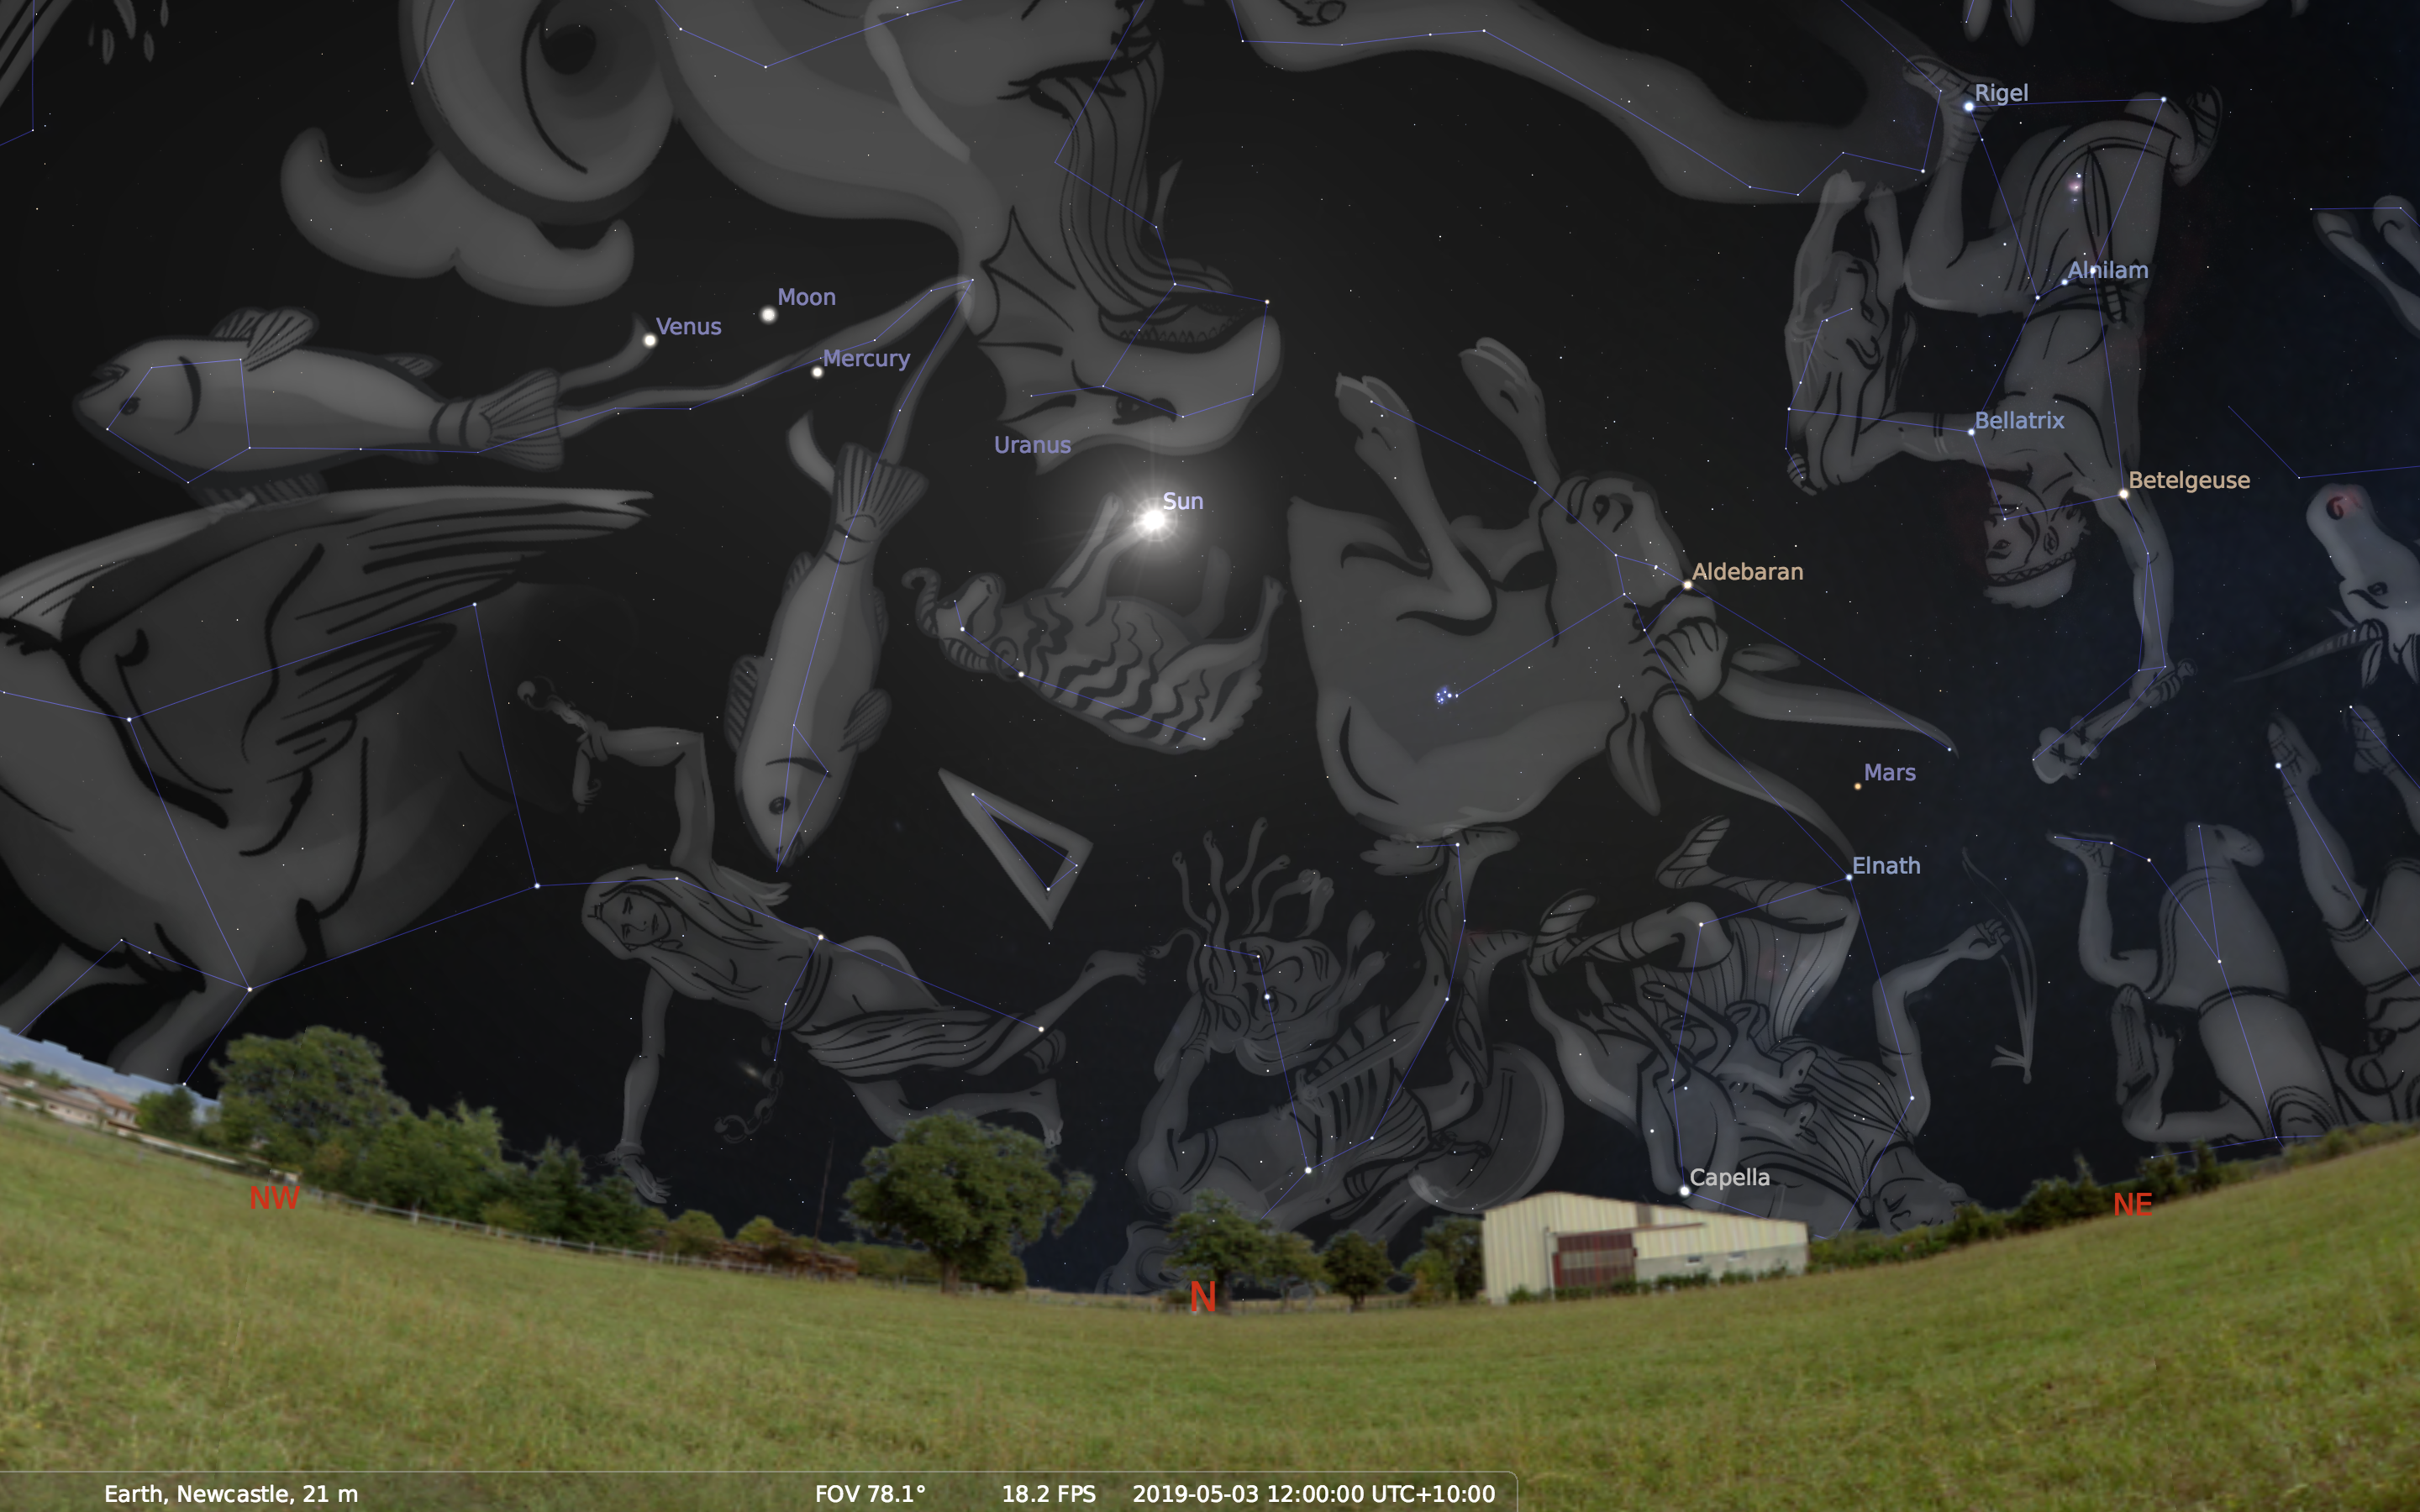
\includegraphics[width=1\columnwidth]{constellation-art}}
	\caption{\label{fig_constellation-art}{Constellation art.}}
\end{figure}


	
